%%%%%%%%%%%%%%%%%%%%%%%%%%%%%%%%%%%%%%%%%
% Journal Article
% LaTeX Template
% Version 1.3 (9/9/13)
%
% This template has been downloaded from:
% http://www.LaTeXTemplates.com
%
% Original author:
% Frits Wenneker (http://www.howtotex.com)
%
% License:
% CC BY-NC-SA 3.0 (http://creativecommons.org/licenses/by-nc-sa/3.0/)
%
%%%%%%%%%%%%%%%%%%%%%%%%%%%%%%%%%%%%%%%%%

%----------------------------------------------------------------------------------------
%	PACKAGES AND OTHER DOCUMENT CONFIGURATIONS
%----------------------------------------------------------------------------------------

\documentclass[twoside]{article}

\usepackage{lipsum} % Package to generate dummy text throughout this template

\usepackage[sc]{mathpazo} % Use the Palatino font
\usepackage[T1]{fontenc} % Use 8-bit encoding that has 256 glyphs
\linespread{1.05} % Line spacing - Palatino needs more space between lines
\usepackage{microtype} % Slightly tweak font spacing for aesthetics

\usepackage[hmarginratio=1:1,top=30mm,columnsep=20pt, hmargin = 2 cm]{geometry} % Document margins
\usepackage{multicol} % Used for the two-column layout of the document
\usepackage[hang, small,labelfont=bf,up,textfont=it,up]{caption} % Custom captions under/above floats in tables or figures
\usepackage{booktabs} % Horizontal rules in tables
\usepackage{float} % Required for tables and figures in the multi-column environment - they need to be placed in specific locations with the [H] (e.g. \begin{table}[H])
\usepackage{hyperref} % For hyperlinks in the PDF

\usepackage{lettrine} % The lettrine is the first enlarged letter at the beginning of the text
\usepackage{paralist} % Used for the compactitem environment which makes bullet points with less space between them

\usepackage{abstract} % Allows abstract customization
\renewcommand{\abstractnamefont}{\normalfont\bfseries} % Set the "Abstract" text to bold
\renewcommand{\abstracttextfont}{\normalfont\small\itshape} % Set the abstract itself to small italic text

\usepackage{titlesec} % Allows customization of titles
\renewcommand\thesection{\Roman{section}} % Roman numerals for the sections
\renewcommand\thesubsection{\Roman{subsection}} % Roman numerals for subsections
\titleformat{\section}[block]{\large\scshape\centering}{\thesection.}{1em}{} % Change the look of the section titles
\titleformat{\subsection}[block]{\large}{\thesubsection.}{1em}{} % Change the look of the section titles

\usepackage{fancyhdr} % Headers and footers
%\pagestyle{fancy} % All pages have headers and footers
%\fancyhead{} % Blank out the default header
\fancyfoot{} % Blank out the default footerz
%\fancyhead[C]{CDT in Delivering Quantum Technologies $\bullet$ December 2015$\bullet$ Vol. XXI, No. 1} % Custom header text
\fancyfoot[RO,LE]{\thepage} % Custom footer text

\usepackage{braket}
\usepackage{amsmath,amsfonts}
\usepackage{hyperref}
\usepackage{tensor}
\usepackage{cancel}
\usepackage{slashed}


\input{../../../UCLCommands.tex}
\usepackage{graphicx}


%----------------------------------------------------------------------------------------
%	TITLE SECTION
%----------------------------------------------------------------------------------------


\iffalse
\title{\vspace{-15mm}\fontsize{24pt}{10pt}\selectfont\textbf{Research Programming - Greengraph}} % Article title

\author{
\large
\textsc{Sofia Qvarfort}\thanks{ }\\[2mm] % Your name
\normalsize CDT in Delivering Quantum Technologies \\
\normalsize Department of Physics and Astronomy, University College London \\ % Your institution
\normalsize \href{sofia.qvarfort.15@ucl.ac.uk}{sofia.qvarfort.15@ucl.ac.uk} \\ % Your email address 
\normalsize \href{GitHub Repository}{GitHub Repository}
\vspace{-5mm}
}
\date{}
\fi

%----------------------------------------------------------------------------------------

%\maketitle % Insert title

\thispagestyle{fancy} % All pages have headers and footers


%%%%%%%%%%%%%%%%%%%%%%%%%%%%%%%%%%%%%%%%%
% Vertical Line Title Page 
% LaTeX Template
% Version 1.0 (27/12/12)
%
% This template has been downloaded from:
% http://www.LaTeXTemplates.com
%
% Original author:
% Peter Wilson (herries.press@earthlink.net)
%
% License:
% CC BY-NC-SA 3.0 (http://creativecommons.org/licenses/by-nc-sa/3.0/)
% 
% Instructions for using this template:
% This title page compiles as is. If you wish to include this title page in 
% another document, you will need to copy everything before 
% \begin{document} into the preamble of your document. The title page is
% then included using \titleGM within your document.
%
%%%%%%%%%%%%%%%%%%%%%%%%%%%%%%%%%%%%%%%%%

%----------------------------------------------------------------------------------------
%	PACKAGES AND OTHER DOCUMENT CONFIGURATIONS
%----------------------------------------------------------------------------------------

%\documentclass{book}

\newcommand*{\plogo}{\fbox{$\mathcal{PL}$}} % Generic publisher logo

%----------------------------------------------------------------------------------------
%	TITLE PAGE
%----------------------------------------------------------------------------------------

\newcommand*{\titleGM}{\begingroup % Create the command for including the title page in the document
\hbox{ % Horizontal box
\hspace*{0.2\textwidth} % Whitespace to the left of the title page
\rule{1pt}{\textheight} % Vertical line
\hspace*{0.05\textwidth} % Whitespace between the vertical line and title page text
\parbox[b]{0.75\textwidth}{ % Paragraph box which restricts text to less than the width of the page


{\noindent\Huge\bfseries  \\[0.5\baselineskip] Greengraph}\\[0.5\baselineskip] % Title

{\noindent\Large\bfseries MPHYG001 -  Python Research Programming }
\\[4\baselineskip] 
{\Large \textsc{Sofia Qvarfort \\  }} % Author name


{\large \textit{Department of Physics and Astronomy, University College London \\[0.5\baselineskip] 
Student. No: SSQVA67 \\[0.5\baselineskip] 
Email: \href{sofia.qvarfort.15@ucl.ac.uk}{sofia.qvarfort.15@ucl.ac.uk}}\\[4\baselineskip] }% Tagline or further description

\vspace{0.5\textheight} % Whitespace between the title block and the publisher
{\noindent 11 January 2016}\\[\baselineskip] % Publisher and logo
}}
\endgroup}

%----------------------------------------------------------------------------------------
%	BLANK DOCUMENT
%----------------------------------------------------------------------------------------

\begin{document}

\pagestyle{empty} % Removes page numbers

\titleGM % This command includes the title page


%----------------------------------------------------------------------------------------
%	ABSTRACT
%----------------------------------------------------------------------------------------


\begin{abstract}
\noindent 
This is a complementary report for the \texttt{greengraph} software package which can be found at \href{https://github.com/sqvarfort/greengraph}{github.com/sqvarfort/greengraph}. \texttt{greengraph} is a package which counts the green pixels in a set number of satellite pictures between two locations. In this report, I outline some of the design choices made while packaging the software as well as the structure used testing framework. Finally, I discuss the advantages and disadvantages of preparing software for distribution and steps one can take to build a user community around \texttt{greengraph} nor any future research programming project. 
\end{abstract}


%----------------------------------------------------------------------------------------
%	ARTICLE CONTENTS
%----------------------------------------------------------------------------------------

\begin{multicols}{2} % Two-column layout throughout the main article text


%------------------------------------------------


\section{Introduction}
The usability and packaging of code is arguably one of the most important aspects when one considers distributing code. In this report, I will outline the design choices and packaging performed for the \texttt{greengraph} code - a tool for counting the number of green pixels found in a series satellite images between two locations. 
I will first outline the functions \texttt{greengraph}, as well as some of the key design choices and automated tests. I will highlight some difficulties encountered, especially focusing on the interaction with the Google Maps API used by \texttt{greengraph}. Towards the end, I discuss the advantages and disadvantages of distributed packaged software in a research programming context, drawing on my own experience of the use of programming in physics. The report is concluded by a short section on what could be improved on in the current project. 





\section{The \texttt{greengraph} code}
The program code was written by Dr. James Hetherington (see \href{http://www.ucl.ac.uk/isd/services/research-it/training/}{http://www.ucl.ac.uk/isd/services/research-it/training/}) and has been packaged and partitioned into two small libraries and a command line interface by the author. Additional files, such as licence and readme files have been added into the repository on GitHub. 


Let us start by looking at what the code does. The greengraph software allows the user to input two locations, one \texttt{start} location and one \texttt{end} location between which the code requests a number of satellite images and counts the number of appearing green pixels. The code makes use of the Google Maps API to fetch satellite images which are subsequently converted into logical arrays denoting which pixels in the image were green. Finally, the number of green pixels is counted and plotted (see example in Fig. \ref{fig:greengraph}). 

The code has been fitted with a simple command line interface that takes three mandatory arguments: \texttt{start}, \texttt{end} and \texttt{filename}, where the filename must include one of the commonly used image file extensions. These are the three fundamental arguments that the code needs in order to run. 



 The code takes three optional arguments: \texttt{---plot}, \texttt{---steps} and \texttt{---delay}.  \texttt{---plot} allows the user to choose whether or not the result of the computation should be immediately plotted using the default graphing software. It is therefore possible to work quickly with several successive inputs without having to bother with closing unwanted pop-up windows. 
 
 


\makebox[0pt][l]{%
\begin{minipage}{\textwidth}
   \fbox{ 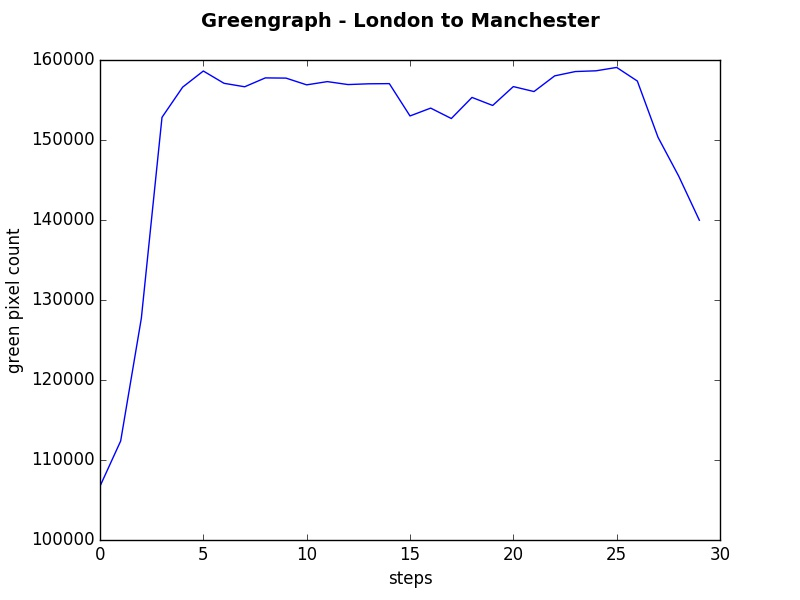
\includegraphics[width=0.4\textwidth]{image.jpg}}
    \captionof{figure}{Example of graph generated by \texttt{greengraph} \\ when run from the command line with \\the inputs \texttt{start = `London'} and \\ \texttt{end = `Manchester'}.}
    \label{fig:greengraph}
\end{minipage}
}

\texttt{---steps} allows the user to choose the number of satellite images taken. A larger step size will mean that the final graph becomes more accurate with more data points. 

\texttt{---delay} is a more specialised function. \href{https://developers.google.com/maps/faq?hl=en#usage_exceed}{According to Google}, the API is limited to 2,500 requests per day, or sending several requests per second from the same IP number. Exceeding this quota or sending too many requests during a short period of time will result in the API returning an error in the form of a picture, which can be seen in Fig. \ref{fig:Google_error}. To avoid overloading the API, the user can input a value \texttt{delay} which will cause the system to pause for \texttt{delay} seconds. Thus, depending on the user's internet connection and other specifications, causing the system to wait before each new request might improve the use of \texttt{greengraph} and prevent graphs from containing invalid data generated from the error image. 


\makebox[0pt][l]{%
\begin{minipage}{\textwidth}
   \fbox{ 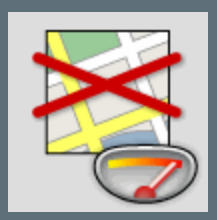
\includegraphics[width=0.3\textwidth]{error_image.png}}
    \captionof{figure}{The error image generated by the Google Maps  \\ API once the request quota has been exceeded. \\ The number of green pixels in this image  \\ is 323. }
    \label{fig:Google_error}
\end{minipage}
}









\section{Design Choices}
In this section, I shall outline some of the design choices made for packaging of the \texttt{greengraph} code. 

\subsection{Partitioning}
Let us begin with the partitioning of the classes. The code has been split into two classes, \texttt{Greengraph} and \texttt{Map}, which can be found in the files \texttt{graph.py} and \texttt{map.py} respectively. This seemed a natural division since the \texttt{Map} class can be used as a module on its own, given that it receives the correct input. 

One difficulty found was choosing in which of these classes to implement new functions. The method \texttt{show\_map} in the \texttt{Greengraph} class uses elements from the \texttt{Map} class, and manipulation of the \texttt{Map} type object, however, we made the choice to let any code interact primarily with the \texttt{Greengraph} objects, from which we can create a \texttt{Map} object, and subsequently access methods in \texttt{Map}. 

\subsection{User Interface}
\texttt{greengraph} can be accessed through a simple command line interface which was described in the previous section. I have strived for retaining as much user freedom as possible, so to allow for both fast and slightly more sophisticated use. I considered making the \texttt{filename} argument optional, however, I am personally not fond of programs that generate additional files without letting me know about so, so effectively `forcing' the user to choose the filename circumvents this problem. 

The step size, which the number of satellite images taken between the \texttt{start} and \texttt{end} locations is an optional argument with a default set to 20. It is an optional argument since one might sometimes require quick results. 

In the same spirit, one might sometimes wish to see quick results, without having to go find the generated file. With that in mind, the option to show the plot as \texttt{---p} has been implemented. Similarly, the option \texttt{---delay} is optional because it might sometimes not be necessary, unless \texttt{--- steps} has been set to a very large number. 

In summary, the following is an example of running \texttt{greengraph} from the command line with all options enabled:  \\[0.5\baselineskip]
\indent \texttt{>>>>greengraph London Manchester } \\
\indent \indent \texttt{greengraph\_image.png -p -s 30 -d 1}



\subsection{Choice of licence}
Following advice on GitHub, I chose to implement the simplest and most open licence as suggested by them, which is the MIT licence. The MIT licence is considered to be the most liberal licence out there. Since the aim a the moment is training and not much else, this was seen as a good choice. More information on the MIT licence can be found \href{http://whatis.techtarget.com/definition/MIT-License-X11-license-or-MIT-X-license}{here}. 




\section{Testing}
In this section, I will outline the testing frameworks used for \texttt{greengraph}. In the moment of writing, there are eight tests for the code which all run successfully with \texttt{nosetests}, as well as code that visualises the maps generated at various stages of the code. In what follows, I will discuss the tests used and some difficulties encountered when designing them. 

\subsection{Testing for bad input}
The code has been fitted with several lines that will catch bad input. For each bad input, a \texttt{ValueError} or \texttt{TypeError} is raised. 

The hardest error to catch was where either the \texttt{start} or \texttt{end} input does not correspond to a location found in Google Maps. According to the \texttt{geopy} documentation, a bad request will return a NoneType object as an error. However, for reasons yet not clear to me, it was not possible to catch this error using an  \texttt{if} statements. Instead, I have used a \texttt{try} statement which catches any \texttt{TypeError}. The code will print an error message and quit the program. However, this exits the program in a different manner compared to all other instances. Style-wise, it is inconsistent, but at least the error is caught. Furthermore, one could also argue that the type of error should be raised as \texttt{NameError} (or similar) instead of a \texttt{TypeError}. Unfortunately, I have not yet found an effective way of changing it. 

Another mention goes to the input to the \texttt{---delay}option. The function \texttt{time.sleep()}, which causes the system to wait for a specified number of seconds, does not currently raise a value error for negative input, but it is a \href{https://bugs.python.org/issue12459}{known issue}. In the meantime, the code has been fitted to raise a ValueError for negative input to \texttt{---delay} by checking the input directly. 

\subsection{Testing calls and API overload}
Further tests prevent the function \texttt{requests} to interact with the internet and checks that the calls were made with correct parameters found in a separate \texttt{fixtures.yml} file. Thus changing any input and running the tests again becomes simple. 

As noticed during testing and building, the Google Maps API has a quota limit for the number of requests that can be sent to it during a short period of time. The API reacts by sending the image seen in Figure \ref{fig:bad_API}, which results in a flat line at $y = 323$ pixels in the graph outputted by  \texttt{greengraph}. 

\makebox[0pt][l]{%
\begin{minipage}{\textwidth}
   \fbox{ 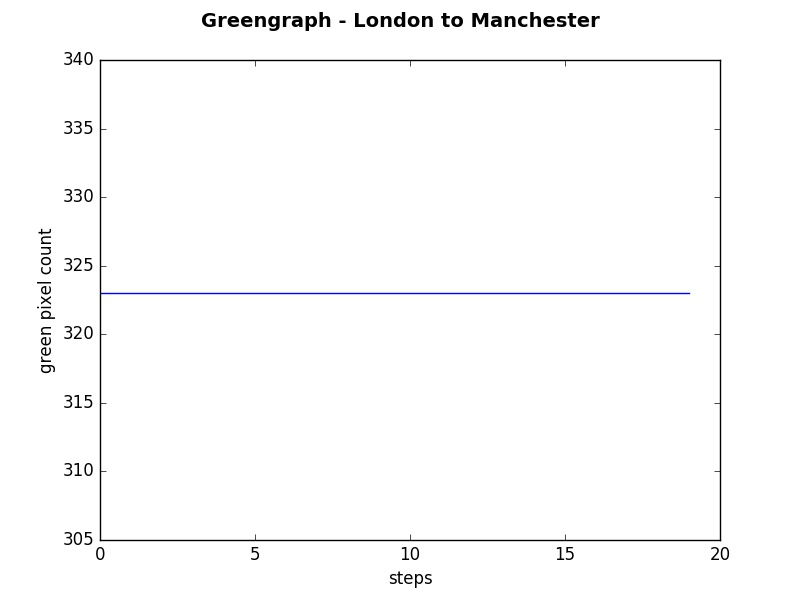
\includegraphics[width=0.4\textwidth]{bad_API.jpg}}
    \captionof{figure}{Example of graph generated by \texttt{greengraph} \\ when the API request quota has been exceeded, \\with the inputs \texttt{start = `London'} and \\ \texttt{end = `Manchester'}.}
    \label{fig:errorimage}
\end{minipage}
}

In order to catch the API overload error, two solutions were considered. \href{https://developers.google.com/maps/documentation/javascript/?csw=1}{Google recommends} that a time delay is added to the loop, such that the API does not receive a high number of requests in a short period of time. Since the request rate will depend on the system in question, it was thought best to make \texttt{---delay} an optional argument such that it can be tailored to the user's need. 

Instead, I chose to implement a simple function that checks when some of the values are equal to 323, which is the number of green pixels in \ref{fig:Google_error}. I chose the threshold value of two and to print a warning instead of quitting the program. The value \texttt{error\_threshold} =2 was chosen because it would be extremely unlikely that two map requests contained a number of 323 green pixels, unless the API limit was hit.  This way, the user will know that data in the graph does not contain  real data, but rather data from the error picture supplied by the API. The program will print a warning instead of exiting, since some of the data could still be of use. 

\subsection{Visualising \texttt{greengraph}}
Naturally, one might like to make sure that the content fetched from the Google Map API actually contains images. I therefore included the file \texttt{visualise\_greengraph.py} into the testing reposetory. This file is not supposed to be run with \texttt{nosetests}, instead it produces the satellite images and the pixel maps of green pixels from the \texttt{sample\_start} and \texttt{sample\_end} entries in the \texttt{fixtures.yml} file. 



\section{Discussion}
In this section, we discuss the advantages and disadvantages of the work related to packaging software into a presentable format. 

\subsection{Advantages and disadvantages of packaging and testing}

\textit{Advantages} One of the advantages of packaging is that the probability of detecting errors significantly increases as the author is forced to think of how the software might be used by an external party. 
Using the framework of licenses and README files also greatly helps others who potentially wish to use the software. Working within this framework saves the author and others from legal obstacles and generally reduces the time spent on administrative matters. 
Furthermore, new users of the software will find it easier to familiarise themselves with the software if the code is structured and simple. By being `user-friendly' the software is also more likely to be spread and used more widely. 

Testing, although not formally required for ease of use, provide a firm foundation for the workings of the code. Any automated tests that are written can easily be run at a later point where, say, the distributed library has been extended. It also makes it possible for contributing authors to check whether their new additions to the original code leave the crucial functions unchanged. 

Making the code user-friendly does not only benefit the intended audience; it may also benefit the author when they return to code after a longer period of time. Any finer details of the usage might not be well-remembered, and thus creating comprehensive user instructions will make it easier to recreate scientific results, for example. 

\textit{Disadvantages} Naturally, the time required to properly package the code is not insignificant. When under pressure to frequently publish, packaging and maintaining code is a time commitment which should not be taken lightly. The learning threshold is fairly steep as well, such that implementing simple tests of imported functions might require significant knowledge of their inner workings. Thus, depending on to which level of testing one requires, more research could be required to find out how appropriate tests might be constructed. In summary, the only disadvantage is the time it would take to neatly package the code. Presumably, one could try and estimate how useful the code will be in the future as well as the size of the user base. For a certain (most likely arbitrary) threshold, the return of packaging might not be very significant. 



\subsection{Community building}
The existence of a user base is invaluable to a developer or research programmer as it will generate feedback on the performance of the code and potentially encourage the author to maintain it. 

Before anything else, any code written for research purposes will be highly specialised. This naturally limits the potential user base, but also provides incentive for the author to think about where their code can be of use outside their field. In physics, many systems are described by a similar set of laws and equations (for example, results in hydrodynamics have been used as underlying material for calculations concerning gravitational waves, see e.g. \href{http://arxiv.org/abs/1103.0373}{this article}). This should act as an incentive to researchers to think broadly about their approach to coding and their field. 

One crucial step towards building a community is choosing the correct software licence. An open and permissive licence, such as the MIT licence chosen for this project permits others to freely use the software. In the context of research programming, this is crucial. Restricting software behind a paywall discourages use, and since many scientist are also good at programming, they might be inclined to find their own solutions instead of paying for the code. 
One could draw a parallel to the rise of the \href{http://arxiv.org/}{arXiv}, where papers are uploaded, albeit without peer review. In spite of this, the arXiv has contributed to spreading scientific ideas and results, as well as circumventing a long and often slow publication pipeline.  Similarly, submitting code to PyPI does not undergo a review process, however the usefulness of the code will establish itself as it becomes easily available through a simple \texttt{pip} command. 

I further believe that being open to user input is crucial to building a strong user community. This can include using the commenting tools on GitHub, or using any other social media platform. Showing that the author cares about further developments and improvements of the code encourages users to get in touch and contribute. This is however also a time commitment that should be carefully taken into account along more pressing research engagements. 


\section{Conclusion}
In this report, I have outlined the functions of \texttt{greengraph} and some of the testing methods used. I concluded that the time required for packaging is not insignificant, but that there exist certain advantages, especially when regarding proliferation of open source software in the research community. 

\section{Further development}
There are a few aspects that I would like to consider for future coding projects. One of them is to better understand the Google Maps API (or any other service) so that the overload error can be avoided. A more sophisticated workaround than the one presented here would be for the program to automatically tune itself to an allowed request rate. Essentially, to write code that interfaces well with any external resource, that resource must be studied to a satisfactory degree. 

A test that I wanted to implement was to input an image into the program and see whether the correct number of pixels was returned. However, under the time constraints I was not able to convert between the relevant file types. A better understanding of the different image formats is needed before that test can be implemented. By doing so, functions such as \texttt{green} in the \texttt{Map} class can be rigorously tested since the input is controlled. 



%------------------------------------------------

\end{multicols}

%----------------------------------------------------------------------------------------
%	REFERENCE LIST
%----------------------------------------------------------------------------------------

\noindent\hrulefill

%----------------------------------------------------------------------------------------

\end{document}
